% To je predloga za poročila o domačih nalogah pri predmetih, katerih
% nosilec je Blaž Zupan. Seveda lahko tudi dodaš kakšen nov, zanimiv
% in uporaben element, ki ga v tej predlogi (še) ni. Več o LaTeX-u izveš na
% spletu, na primer na http://tobi.oetiker.ch/lshort/lshort.pdf.
%
% To predlogo lahko spremeniš v PDF dokument s pomočjo programa
% pdflatex, ki je del standardne instalacije LaTeX programov.

\documentclass[a4paper,11pt]{article}
\usepackage{a4wide}
\usepackage{fullpage}
\usepackage[utf8x]{inputenc}
\usepackage[slovene]{babel}
\selectlanguage{slovene}
\usepackage[toc,page]{appendix}
\usepackage[pdftex]{graphicx} % za slike
\usepackage{setspace}
\usepackage{color}
\definecolor{light-gray}{gray}{0.95}
\usepackage{listings} % za vključevanje kode
\usepackage{hyperref}
\usepackage{amsmath}
\usepackage{graphicx}
\usepackage{epstopdf}
\usepackage{caption}
\usepackage{subcaption}
\renewcommand{\baselinestretch}{1.2} % za boljšo berljivost večji razmak
\renewcommand{\appendixpagename}{Priloge}
\newcommand{\footnoteremember}[2]{
\footnote{#2}
\newcounter{#1}
\setcounter{#1}{\value{footnote}}
}
\newcommand{\footnoterecall}[1]{
\footnotemark[\value{#1}]
}

\lstset{ % nastavitve za izpis kode, sem lahko tudi kaj dodaš/spremeniš
language=Python,
basicstyle=\footnotesize,
basicstyle=\ttfamily\footnotesize\setstretch{1},
backgroundcolor=\color{light-gray},
}

\title{RL competition: Super Mario}
\author{Gregor Majcen (63070199)}
\date{\today}

\begin{document}

\maketitle

\section{Uvod}
Vsi poznamo igrico {\it Super Mario} in tudi večina jo zna igrati. Vendar kaj pa računalnik sam? S pomočjo spodbujevalnega učenja je vse mogoče.

\section{Algoritem}
 Kot glavni algoritem sem izbral ne-deterministično {\bf Q-učenje}. S poskušanjem sem prišel do končne enačbe:
\begin{align}
    alpha_n &= \frac{1}{\text{število obiskov $(s,a)$ do $n$-te iteracije}} \\
    Q_n(s,a) &= (1-alpha_n) * Q_{n-1}(s,a) \nonumber\\&+ alpha_n * ( R(s,a) + R(s',a') + max_{a'}Q_{n-1}(s',a') -  Q_{n-1}(s,a))\\
    Q_n(s[end],a) &= (1-alpha_n) * Q_{n-1}(s,a) \nonumber\\&+ alpha_n * (R(s,a) + R(s,a) -  Q_{n-1}(s,a))
\end{align}

\section{Stanja}
Vsako stanje je določeno v spremenljivki {\it observation}, vendar je zelo preveliko. Zato sem zmanjšal na manjši kvadrat in sicer relativno od pozicijo mario-ta: 4 gor, 4 dol, 5 naprej in 0 nazaj. Temu kvadratu sem dodal še lastnosti pošasti, ki so v manj kot 3 mesta naprej od mario-ta. To stanje sem poimenoval $w$

Zaradi močno zmanjšanega kvadrata je možno, da se stanja ponovijo v zelo različnih okoliščinah sem dodal še eno tabelo stanj $wof$, in sicer: ({\it int(mario.x), int(mario.y), dy, isMonsterNear)}), kjer $dy = [DEC, STD, INC]$ in $isMonsterNear = [True, False]$ glede na to, ali obstaja 3 mesta naprej od mario-ta kakšna pošast.

\section{Akcije}
Na voljo je 12 akcij (kombinacija [-1,1], [0-1], [0-1]). Tudi to sem zaradi hitrejšega učenja skrčil na 7 in sicer: [1, 1, 1], [1, 0, 1], [1, 1, 0], [1, 0, 0], [0, 0, 0], [-1, 0, 0], [-1, 1, 0]. Ostale akcije so se mi zdele odveč, saj jih lahko dosežemo s temi sedmimi. Vse akcije imajo začetno Q oceno 0.

\section{Izbiranje akcije}
V vsakem koraku najprej preberemo oba stanja $w$ in $wof$. Nato najprej pogledamo našo Q tabelo:
\begin{itemize}
\item{$wof$ obstaja:} Poiščemo $argmax_a(Q(wof, a)$, ki je naša zmagovalna akcija. Poglej še, če obstaja $w$, in če ne ga ustvarimo.
\item{$wof$ ne obstaja in $w$ obstaja:} Poiščemo $argmax_a(Q(w, a)$, ki je naša zmagovalna akcija. Nato ocene $w$ prepišemo v $wof$.
\item{$wof$ in $w$ ne obstajata:} Ustvarimo $w$ in $wof$ in izberemo prvo možno akcijo.
\end{itemize}

\section{Dodatne zanimivosti}
\begin{enumerate}
\item Ker želim, da mario čim prej konča, mu pri vsakem premiku naprej prištejem 0.01 (toliko kot izgubi zaradi narejenega koraka).
\item Če se mario zaletava v zid ali kaj podobnega (da sta si dve sosednji stanji enaki): Q(s,a) odštejem 5 (kar močno kaznujem in s tem preprečim, da bi po nepotreben zapravljal čas)
\item Ko mario konča, se pravi se ubije ali pa zmaga, hočem nagraditi njegovo dosedanje delo. Vsem Q(s,a), ki so bile izvajane do $mario.x.end - 10$ prištejem 10, vendar le v primeru, če je prišel dlje kot kadarkoli do sedaj.
\item Ker python funkcija max vzame prvi element, ki je največji, to tudi izkoriščam. Če ima več akcij isto maksimalno oceno, vzame tisto, ki je prva (glej poglavje Akcije).
\end{enumerate}

\section{Rezultati}
\begin{figure}[h]
    \centering
    \begin{subfigure}[b]{0.45\textwidth}
        \centering
        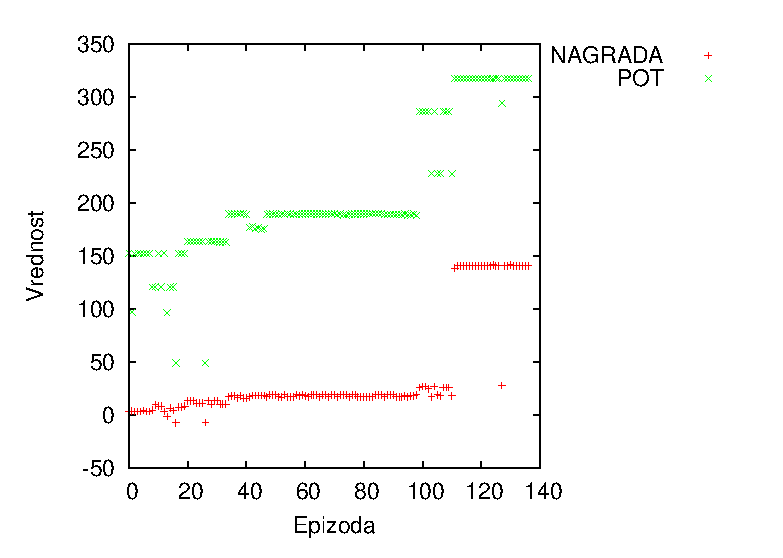
\includegraphics[width=\textwidth]{images/level2.eps}
        \caption{Rezultati druge težavnosti}
    \end{subfigure}
    \begin{subfigure}[b]{0.45\textwidth}
        \centering
        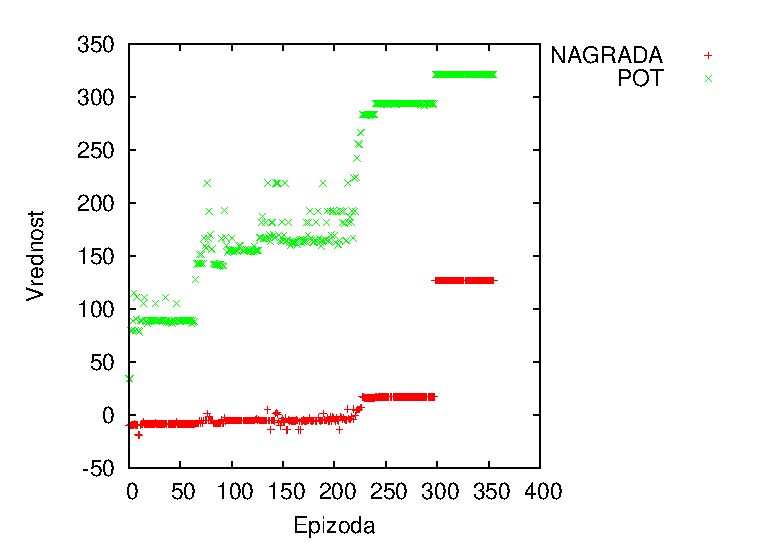
\includegraphics[width=\textwidth]{images/level5.eps}
        \caption{Rezultati pete težavnosti}
    \end{subfigure}
\end{figure}        
\pagebreak

\section{Izjava o izdelavi domače naloge}
Domačo nalogo in pripadajoče programe sem izdelal sam.

\end{document}